\lab{Non-negative Matrix Factorization}{Non-negative Matrix Factorization}

\objective{Understand and implement the non-negative matrix factorization generator for recommendation systems with CVXPY.}

\section*{Introduction}
Collaborative filtering is the process of filtering data for patterns using collaboration techniques.
More specifically, it refers to making prediction about a user's interests based on other users' interests.
These predictions can be used to recommend items and are why collaborative filtering is one of the common methods of creating a recommendation system.

Recommendation systems look at the similarity between users to predict what item a user is most likely to enjoy.
Common recommendation systems include Netflix's "Movies you Might Enjoy" list, Spotify's "Discover Weekly" playlist, and Amazon's "Products You Might Like" suggestions.  


\section*{Non-negative Matrix Factorization}
Non-negative matrix factorization is one algorithm used in collaborative filtering.
It can be applied to many other cases, including image processing, text mining, clustering, and community detection.
The objective of non-negative matrix factorization is to take a non-negative matrix $V$ and factor it into the product of two non-negative matrices. 

For $V\in\mathbb{R}^{m\times n}, 0\preceq W$,


\begin{align*}
\text{minimize}\qquad & ||V-WH|| \\
\text{subject to}\qquad &  0\preceq W, 0\preceq H\\
\text{where}\qquad & W\in\mathbb{R}^{m\times k}, H\in\mathbb{R}^{k\times n}\\
\end{align*}


$k$ is the rank of the decomposition and can either be specified or found using the Root Mean Squared Error (the square root of the MSE), SVD, Non-negative Least Squares, or cross-validation techniques.

For this lab, we will use the Frobenius norm, given by 
\[
||A||_{F} = \sqrt{\sum_{i=1}^{m}\sum_{j=1}^{n} |a|_{ij}^{2}}.
\]

It is equivalent to the square root of the sum of the diagonal of $A^{H}A$.



\begin{problem}
Create the \texttt{NMFRecommender} class, which will be used to implement the NMF algorithm.
Initialize the class with the following parameters: 
\texttt{random\_state} defaulting to $15$,
\texttt{tol} defaulting to $1e-3$, \texttt{maxiter} defaulting to $200$, and \texttt{rank} defaulting to $3$.


Add a method called \texttt{initialize\_matrices} that takes in $m$ and $n$, the dimensions of $V$.
Set the random seed so that initializing the matrices can be replicated:
\begin{lstlisting}
np.random.seed(self.random_state)
\end{lstlisting}
Initialize $W$ and $H$ using randomly generated numbers between 0 and 1, where $W\in\mathbb{R}^{m\times k}$ and $H\in\mathbb{R}^{k\times n}$, where \li{k=rank}.
Store $W$ and $H$ as attributes and return them.
\end{problem}

\section*{CVXPY}
In order to compute the NMF of a matrix we will use the convex optimization package \li{CVXPY}.
\li{CVXPY} is convex optimization package that takes a problem, converts it into standard form, calls a solver, and processes the result.
Here is a basic example of how to use CVXPY
\begin{lstlisting}
import cvxpy as cp

# Create two scalar optimization variables.
x = cp.Variable()
y = cp.Variable()

# Create two constraints.
constraints = [x + y == 1,
               x - y >= 1]

# Form objective.
obj = cp.Minimize((x - y)**2)

# Form and solve problem.
prob = cp.Problem(obj, constraints)
prob.solve()  # Returns the optimal value.

# print the status of the solution
print(prob.status)
\end{lstlisting}
The variables \li{x} and \li{y} are updated as the problem is solved.
Constraints are not required.

Vector valued variables can be created by including the dimension of the variable as an argument like so: \li{x = cp.Variable(10)}.
Similarly matrix valued variables can be created: \li{x = cp.Variable((5,5))}.

When initialized, variables have values of \li{None}.
A value can be assigned to a variable before a problem is solved.
The value can also be extracted after the optimal solution to a problem is found.
\begin{lstlisting}
import numpy as np

random_matrix = np.random.random((5,5))
x = cp.Variable((5,5))
x.value = random_matrix
'''
solve a problem using the variable x
'''
solution_matrix = x.value
\end{lstlisting}



\begin{problem}
Finish the \texttt{NMF} class by adding a method \texttt{fit} that uses CVXPY to find an optimal $W$ and $H$.
It should accept $V$ as a numpy array.

Constructing the problem so that it is known to be convex is important.
Unfortunately, optimizing over 2 matrices being multiplied together breaks the rules of disciplined convex programming.
Because of this, you must solve for $W$ and $H$ alternately. First solve for an optimal $W$ given an $H$, then use that $W$ to solve for an optimal $H$ and so on. Continue until the difference between $W$ and $H$ and their previous values both have a Frobenius norm less than \li{tol}.

Finally, add a method called \li{reconstruct} that reconstructs and returns $V$ by multiplying $W$ and $H$.  

HINT: You can build non-negativity into a \li{CVXPY} variable with \li{x = cp.Variable(n, nonneg=True)}.
You can check if the solution is optimal by checking the status of your problem object with \li{prob.status}.
\end{problem}


\subsection*{Using NMF for Recommendations}

Consider the following marketing problem where we have a list of five grocery store customers and their purchases.
We want to create personalized food recommendations for their next visit. 
We start by creating a matrix representing each person and the number of items they purchased in different grocery categories.
So from the matrix, we can see that John bought two fruits and one sweet.
%
%, where we will try to categorize a customer based on their previous choices and preferences.
%This categorization will help us determine what the customer will want or chose in the future.
%To start off, we have data in the form of labeled columns and rows.
%For example, we could have the customers names as column names and food choices as the row labels.
%The corresponding number is the amount of this type of food that the customer purchased.
%See the following matrix for an example,

\[
V = 
\begin{blockarray}{ccccccc}
  John & Alice & Mary & Greg & Peter & Jennifer \\
  \begin{block}{(cccccc)c}
     0 & 1 & 0 & 1 & 2 & 2 & Vegetables \\
     2 & 3 & 1 & 1 & 2 & 2 & Fruits \\
     1 & 1 & 1 & 0 & 1 & 1 & Sweets \\
     0 & 2 & 3 & 4 & 1 & 1 & Bread \\
     0 & 0 & 0 & 0 & 1 & 0 & Coffee \\
  \end{block}
  \end{blockarray}
\]

After performing NMF on $V$, we'll get the following $W$ and $H$.
\[
W = 
\begin{blockarray}{cccc}
   Component 1 & Component 2 & Component 3\\
  \begin{block}{(ccc)c} 	
	2.19 & 0. & 0.03 & Vegetables\\
	1.53 & 3.13 & 0.11 & Fruits\\
    0.61 & 1.58 & 0. & Sweets\\
    0.01 & 0. & 1.88 & Bread\\
    0.47 & 0.  & 0.  & Coffee\\
   \end{block}
   \end{blockarray}
\]

\[
H = 
\begin{blockarray}{ccccccc}
  John & Alice & Mary & Greg & Peter & Jennifer\\
  \begin{block}{(cccccc)c} 	
   0.  & 0.43 & 0. & 0.42 &  0.96   &   0.86 & Component 1\\
   0.64  & 0.66 & 0.34 & 0. &  0.18   &   0.22 & Component 2\\
   0.  & 1.06 & 1.58 & 2.12 &  0.52   &   0.53 & Component 3\\
   \end{block}
   \end{blockarray}
\]

$W$ represents how much each grocery feature contributes to each component; a higher weight means it's more important to that component.
For example, component $1$ is heavily determined by vegetables followed by fruit, then sweets, coffee and finally bread.
Component $2$ is represented almost entirely by fruits, while component $3$ is based on fruits and bread, with a small amount of vegetables.
$H$ is similar, except instead of showing how much each grocery category affects the component, it shows a much each person belongs to the component, again with a higher weight indicating that the person belongs more in that component.
We can see the John belongs in component $2$, while Jennifer mostly belongs in component 1.

To get our recommendations, we reconstruct $V$ by multiplying $W$ and $H$.

\[
WH = 
\begin{blockarray}{ccccccc}
  John&  Alice  &Mary & Greg & Peter & Jennifer\\
  \begin{block}{(cccccc)c} 	
  0. &  0.9735 & 0.0474 & 0.9834 & 2.118 &   1.8993 &Vegetables\\
      2.0032 & 2.8403 & 1.238 & 0.8758 &  2.0894  &  2.0627 &Fruits\\
      1.0112 & 1.3051 &  0.5372 &  0.2562 &  0.87  &  0.8722 &Sweets\\
       0. & 1.9971 & 2.9704 & 3.9898 & 0.9872 &   1.005 &Bread\\
     0. & 0.2021 & 0. &  0.1974 & 0.4512  &  0.4042 &Coffee\\
   \end{block}
   \end{blockarray}
\]

Most of the zeros from the original $V$ have been filled in.
This is the \li{collaborative filtering} portion of the algorithm.
By sorting each column by weight, we can predict which items are more attractive to the customers.
For instance, Mary has the highest weight for bread at $2.9704$, followed by fruit at $1.238$ and then sweets at $0.5372$.
So we would recommend bread to Mary.

Another way to interpret $WH$ is to look at a feature and determine who is most likely to buy that item.
So if we were having a sale on sweets but only had funds to let three people know, using the reconstructed matrix, we would want to target Alice, John, and Jennifer in that order.
This gives us more information that $V$ alone, which says that everyone except Greg bought one sweet.

\begin{problem}
Use the \texttt{NMFRecommender}  class to run NMF on $V$, defined above, with $2$ components.
Return $W$, $H$, and the number of people who have higher weights in component $2$ than in component $1$.
\end{problem}

\section*{Sklearn NMF}
We also can compute the NMF using SkLearn.
SkLearn uses a similar process as our class above. 
Here rank is represented by the parameter \li{n_components}.
\begin{lstlisting}
from sklearn.decomposition import NMF

model = NMF(n_components=2, init='random', random_state=0)
W = model.fit_transform(V)
H = model.components_
\end{lstlisting}
SkLearn's NMF has other parameters that can also be included and adjusted. The \li{l1_ratio} is a value between 0 and 1 that gives a ratio of how much to weigh the l1 and l2 norms. When \li{l1_ratio} = 1, the l1 norm is used. When \li{l1_ratio} = 0, the l2 norm (Frobenius norm) is used. Any value between 0 and 1 is a weighted combination of the l1 and l2 norms. This ratio helps to prevent the model from over-fitting. The \li{alpha_W} and \li{alpha_H} parameters are floats that represent regularization constants; the default of 0 means that $W$ and $H$ are not regularized. If \li{alpha_H} is not specified, it will take on the value of \li{alpha_W} by default.

\section*{ Endmember Detection using NMF}
NMF can be used for analysis and identification of images. If each image corresponds to a $j \times k$ array of pixel intensities, then the data matrix is constructed by flattening the image into a vector of length $jk$ and using these vectors as the columns of $V$, so $V$ has dimensions $jk \times n$, where $n$ is the number of images to analyze. 
Typically the materials in an image are referred to as the endmembers, which can be thought of as basis images which can be combined to reconstruct any image in the dataset. 
In the NMF decomposition $H[k ,j]$ represents the abundance of the kth endmember or basis face in the jth image. 
$W[:,k]$ represents the spectral signature of the kth endmember. 
Then $V[:,j] \approxeq W H[:,j]$.

\subsection*{Example}
This example exhibits how to use SkLearn's NMF class. The example begins with augmenting and reformatting the images; this will be done for you in the problems following the example. Pay special attention to last two blocks of code which demonstrate using NMF with properly formatted images and plotting the results. 

\begin{lstlisting}
from sklearn.datasets import load_sample_images
import numpy as np

# function to convert colored image to gray scale image
def gray_convert(rgb):
    r, g, b = rgb[:,:,0], rgb[:,:,1], rgb[:,:,2]
    gray = 0.2989 * r + 0.5870 * g + 0.1140 * b
    return gray
    
# load in sample images
dataset = load_sample_images()
# grab the first image
image = dataset.images[0] 
# convert image to gray scale
image = gray_convert(image)

# get augmentations for additional images
flipLR = np.fliplr(image)
flipUP = np.flipud(image)

# create matrix V
images = [np.ravel(image),np.ravel(flipLR),np.ravel(flipUP)]
images = np.transpose(images)

# decompose using NMF
model = NMF(n_components = 5,max_iter = 1000)
W = model.fit_transform(images)
H = model.components_

# plot basis images
plt.subplots_adjust(wspace = .02,hspace = .05)
plt.figure(figsize=(20, 8)) 
for i in range(W.shape[1]):
    plt.subplot(1,5,i+1)
    plt.xticks([], [])
    plt.yticks([],[])
    plt.imshow(np.reshape(W[:,i],(427,640)),cmap = 'gray')

\end{lstlisting}


The following three flattened images now make up the columns of $V$.

\begin{figure}[H]
\centering
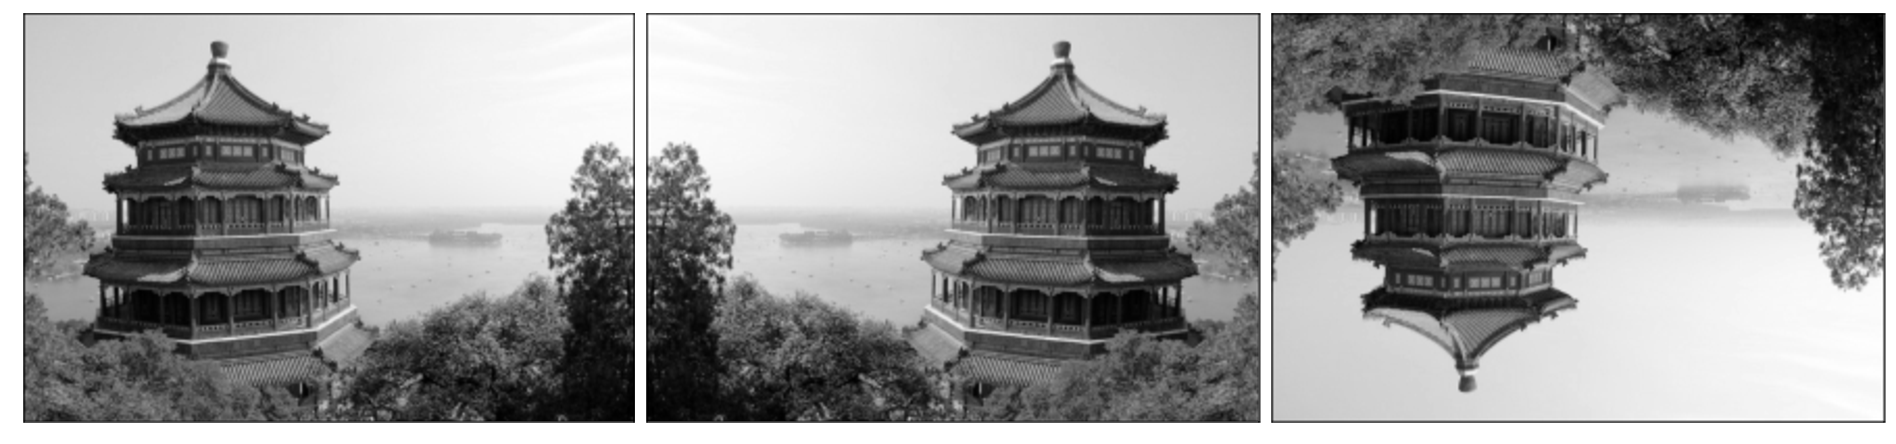
\includegraphics[width=\textwidth]{figures/building_images.pdf}
\caption{Original Images}
\label{fig:basis_faces1}
\end{figure}

Using a rank 5 reconstruction we see that the features used to reconstruct each image deal with the orientation of the building as well as the positive and negative space in each building.
\begin{figure}[H]
\centering
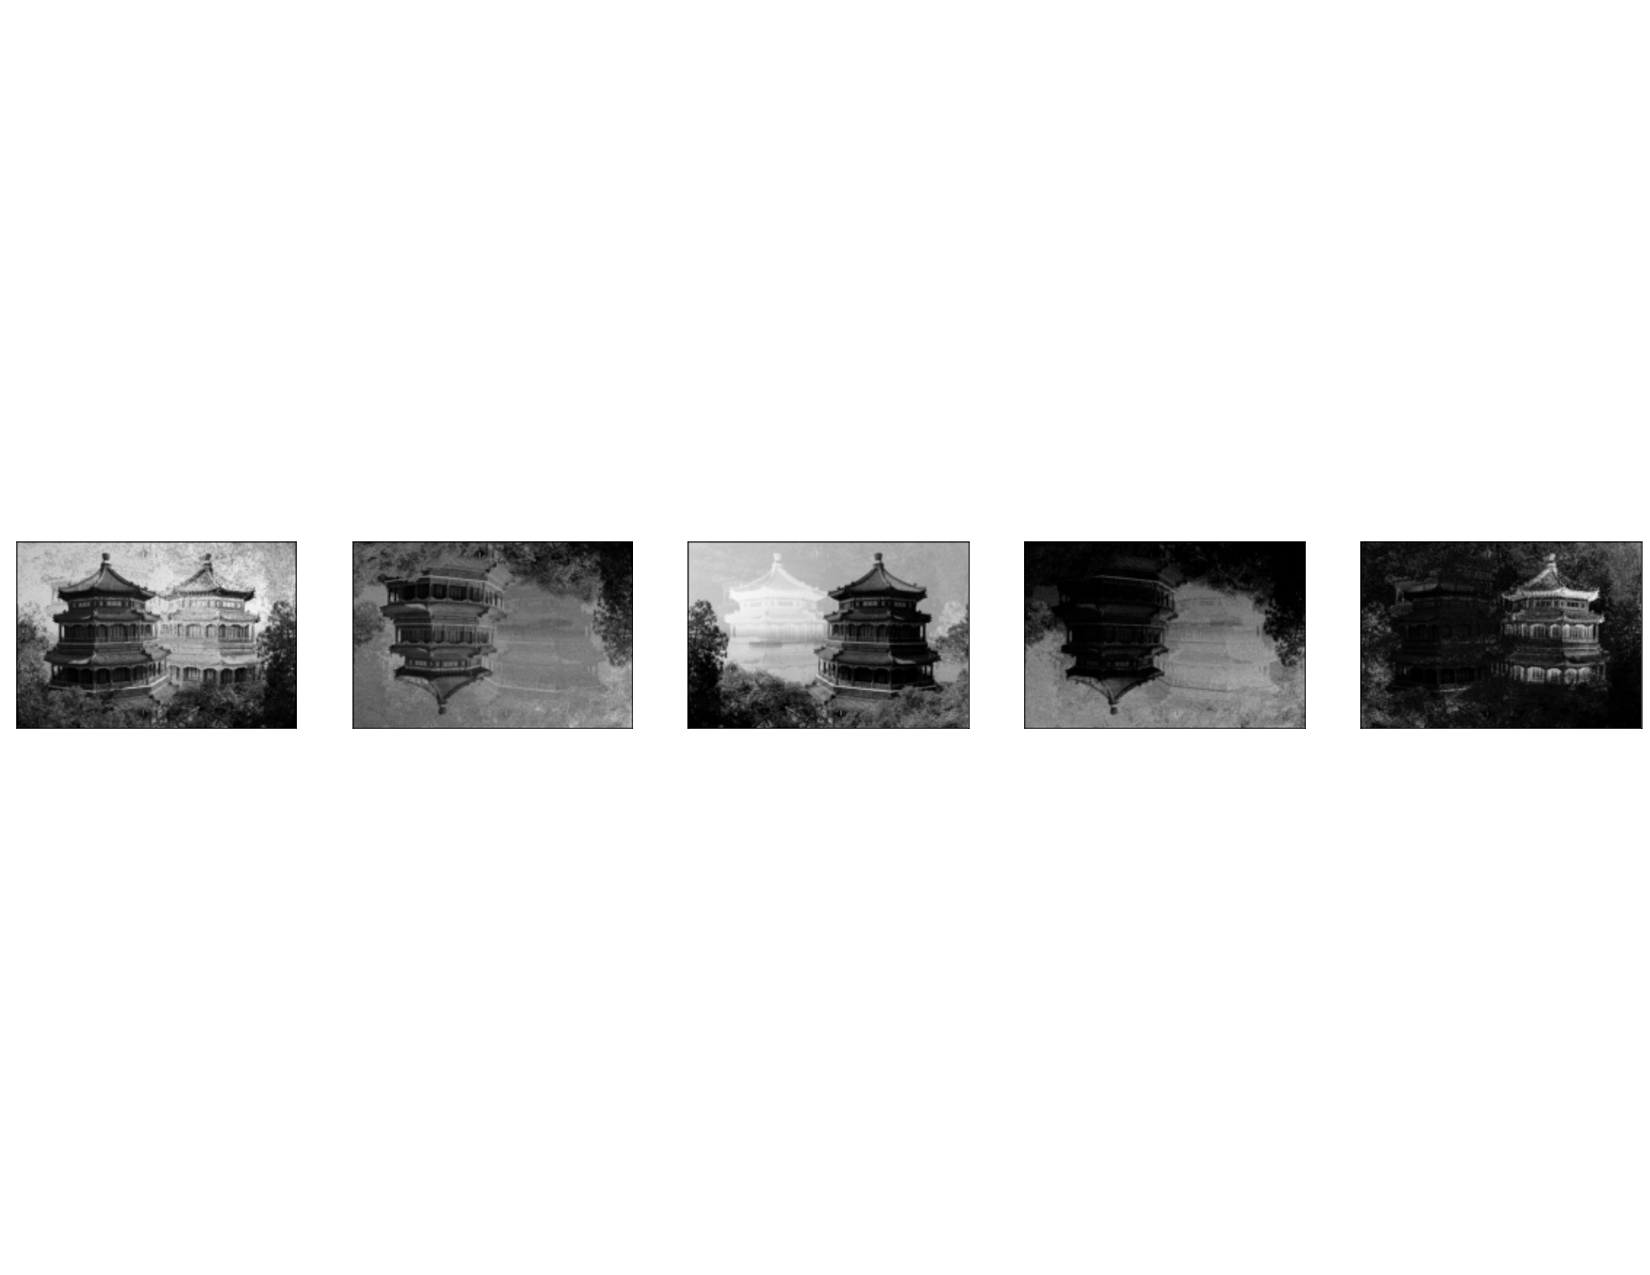
\includegraphics[width=\textwidth]{figures/building_basis_images.pdf}
\caption{Basis images for a rank 5 deconstruction.
	      Each basis image comes from a column of $W$.}
\label{fig:basis_building}
\end{figure}


For the next two problems we will be using a dataset of facial images that we can load in with the code below. Notice that \li{get_faces} formats the faces and returns the $V$ matrix for the face images. 

\begin{lstlisting}
def get_faces(path="./faces94"):
    """Traverse the specified directory to obtain one image per subdirectory. 
        Flatten and convert each image to grayscale.
    
        Parameters:
            path (str): The directory containing the dataset of images.  
    
        Returns:
            ((mn,k) ndarray) An array containing one column vector per
                subdirectory. k is the number of people, and each original
                image is mxn.
        """

    # Traverse the directory and get one image per subdirectory.
    faces = []
    for (dirpath, dirnames, filenames) in os.walk(path):
        for fname in filenames:
            if fname[-3:]=="jpg":       # Only get jpg images.
                # Load the image, convert it to grayscale,
                # and flatten it into a vector.
                faces.append(np.ravel(imread(dirpath+"/"+fname, as_gray=True)))
                break
    # Put all the face vectors column-wise into a matrix.
    return np.transpose(faces)

def show(image, m=200, n=180, plt_show=False):
    """Plot the flattened grayscale 'image' of width 'w' and height 'h'.

    Parameters:
        image ((mn,) ndarray): A flattened image.
        m (int): The original number of rows in the image.
        n (int): The original number of columns in the image.
        plt_show (bool): if True, call plt.show() at the end
    """
    #scale image
    image = image / 255
    #reshape image
    image = np.reshape(image,(m,n))
    #show image
    plt.imshow(image,cmap = "gray")

    if plt_show:
        plt.show()
    
\end{lstlisting}
Similar to the example, we have basis faces that are used to reconstruct the images in the original dataset. 
A sample of basis faces for a rank 75 reconstruction of the faces dataset seem to correspond to the following endmembers: forehead, glasses, hair.

\begin{figure}[H]
\centering
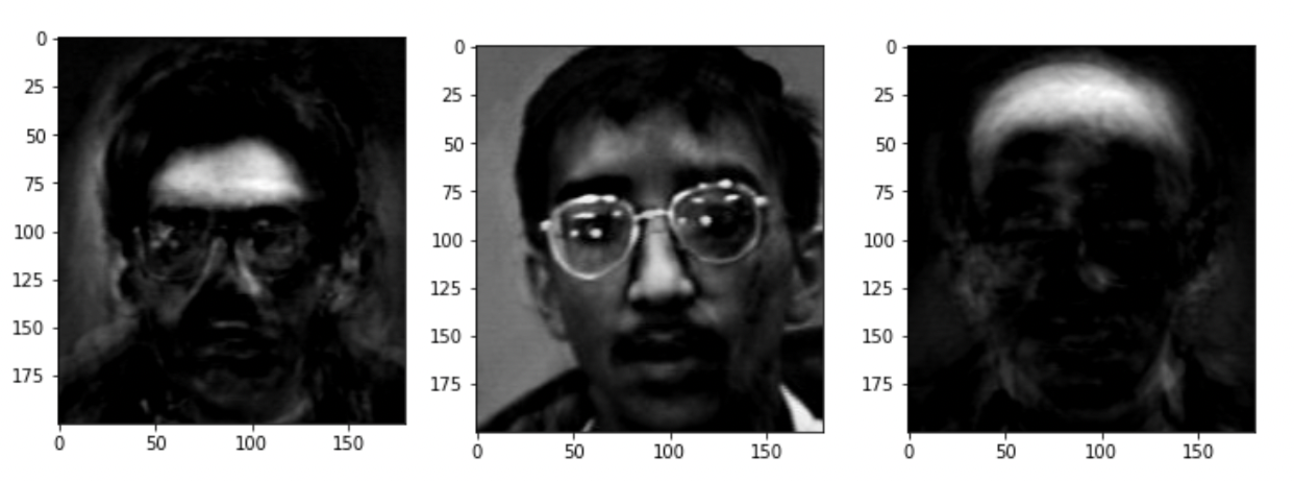
\includegraphics[width=\textwidth]{figures/facial_features.pdf}
\caption{A sample of basis faces.
	      Each basis face comes from a column of $W$.}
\label{fig:basis_faces2}
\end{figure}


\begin{problem}
Load in the facial dataset.
SkLearn has the option to add regularization terms, \li{alpha_W} and \li{l1_ratio}, to the objective function $||V-WH||$.
Reconstruct the third face in the dataset using SkLearn's NMF.
 Perform a grid search over the following:
\li{n\_components} =  [75], \li{alpha_W} = [0, .2, .5], and \li{l1_ratio} = [0, $10^{-5}$, 1]. 

A grid search is a way to hone in on the best parameters by looping through a "grid" of values. It involves running the process for each combination of parameters in the grid. For example, a grid search will run NMF with \li{n\_components} =  75, \li{alpha_W} = 0, and \li{l1_ratio} = 0, then again with  \li{n\_components} =  75, \li{alpha_W} = 0, and \li{l1_ratio} =  $10^{-5}$, and so on, with all combinations of values. Note this will take a while to run (approximately 10 minutes) since it will run and fit the NMF model 9 total times. In the NMF function, make sure to set \li{init = "random"} or else the function won't converge correctly.

Determine which set of parameters best reconstructs the face. These are the parameters that most closely approximate the third face with $W$ and $H$. (Hint: For each set of parameters, find the norm of \li{faces[:,2] - W @ H[:,2]} and see which is the smallest. Due to the randomness of the algorithm, answers may vary. Additionally, notice how we only look at the third face to avoid large matrix multiplication, which is computationally expensive.)

Plot all reconstructions of the third face and put the parameters in the title; use subplots.
\end{problem}

\begin{problem}
Run NMF on the facial dataset again, using the best parameters from the problem above.
Next, for the second and twelfth faces in the dataset, find the 10 basis faces with the largest coefficients. 
Plot these basis faces along with the original image using subplots.
In a markdown block write a sentence or two about differences you notice in the features of the basis faces (look closely).
\end{problem}
